\chapter{电化学电池的热力学}\label{ch:b2:cell-thermodynamics}

一辆氢燃料电池公交车的电堆由几百个薄电池组成。在每个电池中，
氢气与空气中的氧气无需火焰即可化合生成水，
能量以电流的形式释放出来。决定这类电堆性能的有两个数，
二者都直接来自\omterm{def:b2:reaction-free-energy:gibbs-energy}{吉布斯自由能}表：任何电池的电压都不能超过
\qty{1.23}{V}，而无论多理想的燃料电池，都不能把其中氢的全部能量
转化为电功。本章将电池电压与其反应的\omterm{def:b2:reaction-free-energy:gibbs-energy}{吉布斯自由能}联系起来，
推导本科一年级分册已使用的能斯特方程，
并借助电压表和
温度计读取反应的熵与焓。

\begin{recall}
本科一年级分册内容：电池、半电池、阳极与阴极、盐桥、电池
电压、电极电势、标准电极电势与标准氢电极、
能斯特方程（该分册中已承认）、由电势求平衡常数。
\Cref{ch:b2:reaction-free-energy}：$\Delta_r G$、$\Delta_r G^\circ$
与 $\Delta_r G = \Delta_r G^\circ + RT\ln Q$；反应方向判据。
\Cref{ch:b2:chemical-potential}：活度。第 1 册内容：电解。
\end{recall}

\begin{omfigure}
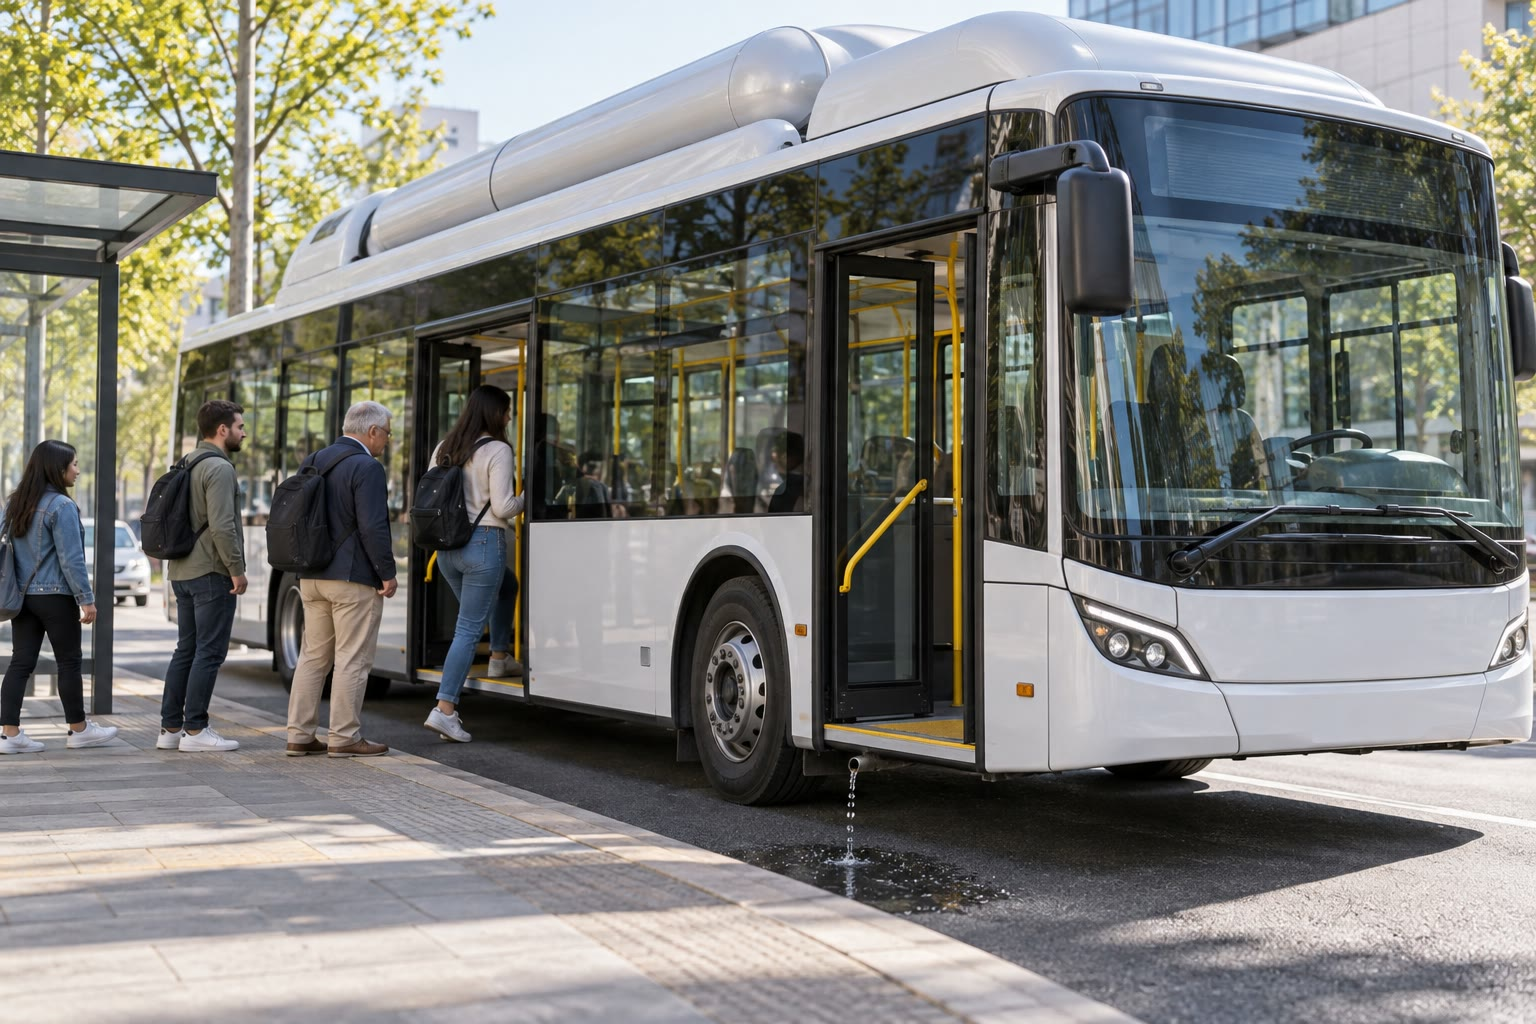
\includegraphics[width=0.62\linewidth]{images/book3/ai/b2-09-fuel-cell-bus.jpg}

{\small 停在站点的氢燃料电池公交车：氢气储罐位于
车顶整流罩下方，唯一的排放物是水，水滴落在车身下方。}
\end{omfigure}

\section{电功与法拉第常数}

\begin{definition}[法拉第常数]\label{def:b2:cell-thermodynamics:faraday}
\emph{法拉第常数}\index{法拉第常数}是
1 摩尔元电荷所带的电荷量，$F = N_A e = \qty{96485.33}{C/mol}$。
% ledger: const:F
\end{definition}

\begin{proposition}[通过的电荷]\label{prop:b2:cell-thermodynamics:charge}
若电池反应按交换 $n$ 个电子的方式书写，其反应进度推进
$\Delta\xi$，则流经外电路的电荷为 $Q =
nF\,\Delta\xi$。
\end{proposition}

\begin{proof}
反应进度 $\Delta\xi$ 使 $n\,\Delta\xi$ 摩尔电子由
经导线由阳极转移至阴极，每个电子的电荷量绝对值为 $e$：
$Q = n\,\Delta\xi\,N_A e$。
\end{proof}

当电荷 $Q$ 在电压 $U$ 驱动下通过电路时，电路所获得的功
为 $QU$。从提供该功的电池来看，
电池所获得的电功为 $\delta W_{\text{el}} = -U\,\delta Q = -nFU\,
d\xi$。

\begin{omfigure}
\begin{tikzpicture}[font=\small, >={Stealth}]
  \draw[thick, rounded corners, fill=omDef!8] (0,0) rectangle (3.2,2.2);
  \node[align=center] at (1.6,1.1) {电池（系统）\\ 反应 $d\xi$};
  \draw[->, thick, omThm] (3.2,1.6) -- (5.6,1.6) node[right, align=left] {输出的 $\delta W_{\text{el}}$\\ $= nFU\,d\xi$};
  \draw[->, thick, omDef] (5.6,0.6) -- (3.2,0.6) node[pos=0, right, align=left] {吸收的 $\delta Q_{\text{热}}$\\ （正负均可）};
  \draw[<->, thick] (1.6,2.2) -- (1.6,3.0) node[above] {$T$、$p$ 下的外界};
\end{tikzpicture}

{\small 恒温恒压下的电池作为热力学系统：
它与外界交换热量，并通过
外电路输出电功。采用第一定律的符号约定（功与吸热均取正值），
$\delta W_{\text{el}} = -nFU\,d\xi$。}
\end{omfigure}

\section{电池反应的吉布斯自由能}

\begin{theorem}[电功与吉布斯自由能]\label{thm:b2:cell-thermodynamics:delta-g-nfe}
电池在恒定 $T$、$p$ 下工作时，所输出的电功至多
等于其\omterm{def:b2:reaction-free-energy:gibbs-energy}{吉布斯自由能}的减少量：对于进度 $d\xi$，
$nFU\,d\xi \leq -\Delta_r G\,d\xi$。当电池可逆工作（
电流无限小）时等号成立，电池电压即为
电动势
\[
  \Delta_r G = -nFE .
\]
\end{theorem}

\begin{proof}
恒压下的第一定律，并将体积功分离出来：
$dH = \delta Q + \delta W_{\text{el}}$。第二定律：$dS \geq \delta Q/T$。在
$T$、$p$ 恒定时，$dG = dH - T\,dS \leq \delta W_{\text{el}} = -nFU\,d\xi$。
由 $dG = \Delta_r G\,d\xi$ 得 $\Delta_r G\,d\xi \leq -nFU\,d\xi$，
即 $nFU\,d\xi \leq -\Delta_r G\,d\xi$。对可逆过程，第二定律中的不等式
取等号，此时无
电流时测得的电压为 $E$：$\Delta_r G = -nFE$。
\end{proof}

因此，电池要正向进行（$d\xi > 0$，对外输出功），只有当 $\Delta_r G <
0$，即 $E > 0$，且正负极的选取使所写反应
自阳极流向阴极。有电流通过的实际电池所输出的功
小于 $-\Delta_r G$，其差值以热的形式在
内阻和电极处耗散（见\cref{ch:b2:current-potential-curves}）。

\begin{example}[丹尼尔电池]\label{ex:b2:cell-thermodynamics:daniell}
对于 \ce{Zn + Cu^2+ -> Zn^2+ + Cu}，$\Delta_r G^\circ = \Delta_f G^\circ(\ce{Zn^2+}) -
\Delta_f G^\circ(\ce{Cu^2+}) = -147.06 - 65.49 = \qty{-212.55}{kJ/mol}$，且 $n = 2$：
$E^\circ = 212\,550/(2 \times 96\,485) = \qty{1.10}{V}$，即标准条件下
丹尼尔电池的测量电压。
% ledger: dfg:Zn2+_ao, dfg:Cu2+_ao, const:F, emf:Daniell
\end{example}

\section{能斯特方程与标准电极电势}

本科一年级分册中已承认能斯特方程；现由
$\Delta_r G = \Delta_r G^\circ + RT\ln Q$ 推出。

\begin{theorem}[能斯特方程的推导]\label{thm:b2:cell-thermodynamics:nernst-derived}
对于半反应 $\alpha\,\mathrm{Ox} + n\,\mathrm e^- \rightleftharpoons
\beta\,\mathrm{Red}$，电极在温度 $T$ 下的电势为
\[
  E = E^\circ + \frac{RT}{nF}\ln\frac{a_{\mathrm{Ox}}^{\alpha}}{a_{\mathrm{Red}}^{\beta}} ,
\]
式中的活度包括半反应中其余各物种的活度
（\ce{H+} 计入，水除外），各以其化学计量数为指数。
\end{theorem}

\begin{proof}
电极的电势是由标准
氢电极（阳极）与该电极（阴极）组成的电池的电压，其反应为
\[
  \alpha\,\mathrm{Ox} + \tfrac n2\,\ce{H2} \longrightarrow \beta\,\mathrm{Red} + n\,\ce{H+} ,
\]
其反应商中，在标准氢电极处取 $a_{\ce{H+}} = 1$、$p_{\ce{H2}} = p^\circ$，
反应商化简为 $a_{\mathrm{Red}}^\beta/
a_{\mathrm{Ox}}^\alpha$。由\cref{thm:b2:cell-thermodynamics:delta-g-nfe}，
$E = -\Delta_r G/(nF) = -\Delta_r G^\circ/(nF) - (RT/nF)\ln Q$；取 $E^\circ =
-\Delta_r G^\circ/(nF)$，即得上式。在 \qty{298.15}{K} 下，$RT\ln 10/F =
\qty{0.0592}{V}$。
\end{proof}

\begin{proposition}[由吉布斯自由能求标准电极电势]\label{prop:b2:cell-thermodynamics:standard-potential}
约定 $\Delta_f G^\circ(\ce{H+}, \text{aq}) = 0$ 且
$\Delta_f G^\circ(\ce{H2}, \text{g}) = 0$，则电对的标准电极电势为
$E^\circ = -\Delta_r G^\circ/(nF)$，其中 $\Delta_r G^\circ$ 为按还原方向书写的
半反应的标准\omterm{def:b2:reaction-free-energy:gibbs-energy}{吉布斯自由能}，并将电子的
\omterm{def:b2:reaction-free-energy:gibbs-energy}{吉布斯自由能}取为零。
\end{proposition}

\begin{proof}
在与氢电极构成的反应中，$\tfrac n2\,\ce{H2}$ 与
$n\,\ce{H+}$ 在上述约定下对 $\Delta_r G^\circ$ 均无贡献：
故电池反应的标准\omterm{def:b2:reaction-free-energy:gibbs-energy}{吉布斯自由能}即为该半反应的标准\omterm{def:b2:reaction-free-energy:gibbs-energy}{吉布斯自由能}。
\end{proof}

\begin{method}[由数据表求标准电极电势]\label{met:b2:cell-thermodynamics:e-from-gibbs}
\begin{enumerate}
  \item 将半反应按还原方向书写，用 \ce{H+} 和
        \ce{H2O} 配平，电子数为 $n$。
  \item 计算 $\Delta_r G^\circ = \sum\nu_i\Delta_f G^\circ_i$（生成物
        取正号），单质、\ce{H+} 和电子的取值均为零。
  \item $E^\circ = -\Delta_r G^\circ/(nF)$，单位为伏特，$\Delta_r G^\circ$ 的单位为
        焦耳每摩尔。
\end{enumerate}
\end{method}

\begin{example}[氯化银电极]\label{ex:b2:cell-thermodynamics:agcl}
\ce{AgCl(s) + e- -> Ag(s) + Cl^-}：$\Delta_r G^\circ = -131.228 - (-109.789) =
\qty{-21.439}{kJ/mol}$，$E^\circ = 21\,439/96\,485 = \qty{0.222}{V}$。其电势
仅取决于氯离子活度：在饱和氯化钾
溶液中，它是稳定的参比电极。
% ledger: dfg:Cl-_ao, dfg:AgCl_cr
\end{example}

\begin{proposition}[电极电势的组合]\label{prop:b2:cell-thermodynamics:combining}
若半反应 (3)（电子数为 $n_3$）是半反应 (1)
与半反应 (2) 之和（电子数分别为 $n_1$ 和 $n_2$），则
\[
  n_3E_3^\circ = n_1E_1^\circ + n_2E_2^\circ ;
\]
电势本身不可相加。
\end{proposition}

\begin{proof}
标准\omterm{def:b2:reaction-free-energy:gibbs-energy}{吉布斯自由能}可加，即 $\Delta_r G_3^\circ = \Delta_r G_1^\circ + \Delta_r
G_2^\circ$，电子数亦相加，$n_3 = n_1 + n_2$。将各 $\Delta_r
G^\circ$ 除以 $-F$。
\end{proof}

\begin{example}[铁的两种氧化态]\label{ex:b2:cell-thermodynamics:iron}
\ce{Fe^3+ + e- -> Fe^2+} 的 $E^\circ = (-78.90 + 4.7)/(-96.485) = \qty{0.77}{V}$，
而 \ce{Fe^2+ + 2e- -> Fe} 的 $E^\circ = -78.90/(2 \times 96.485) =
\qty{-0.41}{V}$。由此 \ce{Fe^3+ + 3e- -> Fe}：$E^\circ = (0.77 - 0.82)/3 =
\qty{-0.02}{V}$，并非两者之和。
% ledger: dfg:Fe2+_ao, dfg:Fe3+_ao
\end{example}

\section{温度、熵与燃料电池的效率}

\begin{definition}[温度系数]\label{def:b2:cell-thermodynamics:temperature-coefficient}
称电池的\emph{温度系数}\index{温度系数}为
其电动势对温度的导数
$(\partial E/\partial T)_p$。
\end{definition}

\begin{proposition}[由电池数据求熵与焓]\label{prop:b2:cell-thermodynamics:entropy}
对于标准电池反应，
\[
  \Delta_r S^\circ = nF\,\frac{dE^\circ}{dT}, \qquad
  \Delta_r H^\circ = -nF\Big(E^\circ - T\frac{dE^\circ}{dT}\Big),
\]
且电池在温度 $T$ 下可逆工作时，
自外界吸收的热量为每摩尔反应 $T\Delta_r S$。
\end{proposition}

\begin{proof}
$\Delta_r S^\circ = -d\Delta_r G^\circ/dT$（由 $dG = -S\,dT + V\,dp$，对
$\xi$ 求导）$= nF\,dE^\circ/dT$；再由 $\Delta_r H^\circ = \Delta_r G^\circ
+ T\Delta_r S^\circ$。对可逆变化，$\delta Q = T\,dS = T\Delta_r S\,
d\xi$。
\end{proof}

\begin{method}[由电池数据求反应的热力学量]\label{met:b2:cell-thermodynamics:cell-data}
\begin{enumerate}
  \item 在若干温度下测量 $E$；斜率即为 $dE/dT$。
  \item $\Delta_r G = -nFE$，$\Delta_r S = nF\,dE/dT$，$\Delta_r H = \Delta_r G +
        T\Delta_r S$。
  \item 电池可逆工作时，每摩尔交换的热量为 $T\Delta_r S$；
        若电池以电压 $U < E$ 输出电流，则释放的热量为
        每摩尔 $-\Delta_r H - nFU$。
\end{enumerate}
\end{method}

对于生成液态水的氢–氧电池，CODATA 的关键数值
给出 $\Delta_r H^\circ = \qty{-285.83}{kJ/mol}$，
\[
  \Delta_r S^\circ = 69.95 - 130.68 - \tfrac12 \times 205.15 = \qty{-163.3}{J/(K.mol)} ,
\]
于是 $\Delta_r G^\circ = \qty{-237.14}{kJ/mol}$，且 $E^\circ = \qty{1.229}{V}$；
\omterm{def:b2:cell-thermodynamics:temperature-coefficient}{温度系数}为 $\Delta_r S^\circ/(2F) = \qty{-0.85}{mV/K}$。氢燃料电池在
高温下输出的电压低于低温时。
% ledger: dfh:H2O-l, s0:H2O_l, s0:H2_g, s0:O2_g, janafG:H2O_l.298

\begin{omfigure}
\begin{tikzpicture}
\begin{axis}[width=0.48\linewidth, height=5.4cm, xmin=280, xmax=1020,
  ymin=0.95, ymax=1.26, axis x line=bottom, axis y line=left,
  xlabel={$T$ (K)}, ylabel={$E^\circ$ (V)}, tick label style={font=\small},
  label style={font=\small}, title={\small 标准电压}]
\addplot[omDef, thick, mark=*, mark size=1.2pt] table[x=T, y=E] {figdata/out/bachelor-2-cell-thermodynamics-a-liquid.dat};
\addplot[omThm, thick, mark=*, mark size=1.2pt] table[x=T, y=E] {figdata/out/bachelor-2-cell-thermodynamics-a-gas.dat};
\node[font=\scriptsize, omDef, anchor=north east] at (axis cs:480,1.05) {液态水};
\node[font=\scriptsize, omThm, anchor=south west] at (axis cs:560,1.12) {水蒸气};
\end{axis}
\end{tikzpicture}\hfill
\begin{tikzpicture}
\begin{axis}[width=0.48\linewidth, height=5.4cm, xmin=280, xmax=1520,
  ymin=0, ymax=1.0, axis x line=bottom, axis y line=left,
  xlabel={$T$ (K)}, ylabel={效率}, tick label style={font=\small},
  label style={font=\small}, title={\small 最大效率}]
\addplot[omThm, thick, mark=*, mark size=1.2pt] table[x=T, y=eta] {figdata/out/bachelor-2-cell-thermodynamics-b.dat};
\addplot[black!60, thick, dashed] table[x=T, y=eta] {figdata/out/bachelor-2-cell-thermodynamics-b-carnot.dat};
\node[font=\scriptsize, omThm, anchor=south] at (axis cs:700,0.87) {燃料电池};
\node[font=\scriptsize, black!70, anchor=north west] at (axis cs:520,0.40) {卡诺，$T_0 = \qty{298}{K}$};
\end{axis}
\end{tikzpicture}

{\small 来自 JANAF 表的氢–氧电池。左图：标准电压
$-\Delta_r G^\circ/(2F)$，对应液态水（温度可至 \qty{500}{K}，液体保持
在其标准状态下）与水蒸气情形。右图：最大效率
$\Delta_r G^\circ/\Delta_r H^\circ$，即生成水蒸气的电池的
与在 $T$ 和 \qty{298}{K} 之间工作的热机的卡诺效率相比较；
只有在约 \qty{1150}{K} 以上，热机才更优。}
% ledger: janafG:H2O_l.298, janafG:H2O_l.300, janafG:H2O_l.400, janafG:H2O_l.500, janafG:H2O.298, janafG:H2O.300, janafG:H2O.400, janafG:H2O.500, janafG:H2O.600, janafG:H2O.700, janafG:H2O.800, janafG:H2O.900, janafG:H2O.1000, janafdfH:H2O_g.300, janafdfH:H2O_g.400, janafdfH:H2O_g.500, janafdfH:H2O_g.600, janafdfH:H2O_g.700, janafdfH:H2O_g.800, janafdfH:H2O_g.900, janafdfH:H2O_g.1000, janafdfH:H2O_g.1100, janafdfH:H2O_g.1300, janafdfH:H2O_g.1500, janafG:H2O.1100, janafG:H2O.1300, janafG:H2O.1500
\end{omfigure}

\begin{definition}[燃料电池的热力学效率]\label{def:b2:cell-thermodynamics:efficiency}
称燃料电池的\emph{热力学效率}\index{热力学效率}为
其输出的电功与燃料在同温度下燃烧释放的热量之比，
即每摩尔 $-\Delta_r H$。
\end{definition}

\begin{proposition}[燃料电池的最大效率]\label{prop:b2:cell-thermodynamics:efficiency}
燃料电池的\omterm{def:b2:cell-thermodynamics:efficiency}{热力学效率}至多为 $\Delta_r G/\Delta_r H$，
在可逆工作时取到此上界，在工作电压下等于 $(nFU)/(-\Delta_r H)$，
其中 $U$ 为工作电压。与热机不同，
它不受卡诺效率 $1 - T_0/T$ 的限制。
\end{proposition}

\begin{proof}
由\cref{thm:b2:cell-thermodynamics:delta-g-nfe}可知，每摩尔的功为 $nFU \leq
-\Delta_r G$，两边除以 $-\Delta_r H$。电池在单一温度下将化学能直接
转化为功：不从热源吸热、再将部分热量传给冷源，
因此卡诺界限（它只针对此类循环）
并不适用。其自身的界限由 $T\Delta_r S$ 决定，即
可逆电池必须交换的热量。
\end{proof}

\begin{omfigure}
\begin{tikzpicture}[font=\small, x=0.022cm, y=0.6cm]
  \draw[->] (0,0) -- (320,0) node[right, font=\scriptsize] {\unit{kJ/mol}};
  \foreach \v in {0,100,200,300} \draw (\v,0) -- (\v,-0.12) node[below, font=\scriptsize] {\v};
  \fill[omThm!70] (0,2.2) rectangle (285.83,2.8);
  \node[anchor=west, font=\scriptsize] at (290,2.5) {$-\Delta_r H^\circ = 285.8$：燃烧热};
  \fill[omDef!70] (0,1.2) rectangle (237.14,1.8);
  \fill[omProp!70] (237.14,1.2) rectangle (285.83,1.8);
  \node[anchor=west, font=\scriptsize] at (290,1.5) {$-\Delta_r G^\circ = 237.1$ 功 $+$ $48.7$ 热量};
  \fill[omDef!40] (0,0.2) rectangle (135.1,0.8);
  \fill[omProp!40] (135.1,0.2) rectangle (285.83,0.8);
  \node[anchor=west, font=\scriptsize] at (290,0.5) {在 \qty{0.70}{V} 下：$135.1$ 功 $+$ $150.7$ 热量};
\end{tikzpicture}

{\small 在燃料电池中，一摩尔氢气的能量去向
（温度 \qty{298}{K}，液态水）。上图：明火燃烧会释放的热量。中图：
可逆电池须以热量形式放出 $-T\Delta_r S^\circ = \qty{48.7}{kJ}$，
无论其设计如何。下图：实际电池在 \qty{0.70}{V} 下工作。}
% ledger: dfh:H2O-l, s0:H2O_l, s0:H2_g, s0:O2_g, const:F
\end{omfigure}

\begin{history}[法拉第电解定律]
\begin{minipage}[t]{0.27\linewidth}
\vspace{0pt}
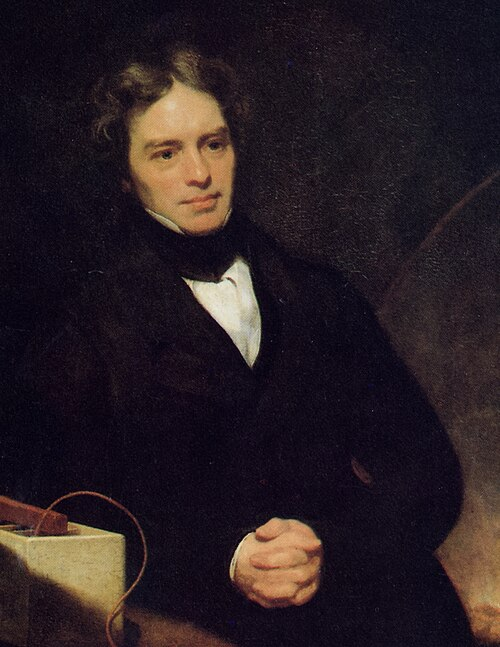
\includegraphics[width=\linewidth]{images/book3/faraday.jpg}
\end{minipage}\hfill
\begin{minipage}[t]{0.69\linewidth}
\vspace{0pt}
1834 年，法拉第以自己设计的
电量计测量电解产物，并指出：电极上生成的
物质质量与通过的电量成正比，并且
当通过的电量相同时，不同物质的质量
之比等于它们的化学当量之比。他创造了
电极、阳极、阴极、离子、阴离子和阳离子等词。以他的名字命名的常数
使这些定律化为 $Q = nF\,\Delta\xi$。（肖像作者：托马斯·菲利普斯，
1842 年，公有领域，维基共享资源。）
\end{minipage}
\end{history}

\section{浓差电池}

\begin{definition}[浓差电池]\label{def:b2:cell-thermodynamics:concentration-cell}
称\emph{浓差电池}\index{浓差电池}为由两个同一电对的
半电池组成、且二者仅在某一物种的浓度（或
压强）上有所不同。
\end{definition}

\begin{proposition}[浓差电池的电压]\label{prop:b2:cell-thermodynamics:concentration-cell}
金属 M 的两个电极分别浸入 \ce{M^{n+}} 的溶液中，其浓度分别为
$c_1 < c_2$，经盐桥相连，得到电压
\[
  U = \frac{RT}{nF}\ln\frac{c_2}{c_1} ,
\]
浓度较大的一侧为正极。电池工作直至
两侧浓度相等为止。
\end{proposition}

\begin{proof}
由能斯特方程，每个电极的电势为 $E_i = E^\circ + (RT/nF)\ln c_i$（\omterm{def:b2:chemical-potential:ideal-mixture}{理想
稀溶液}）；$E^\circ$ 在作差时抵消。反应为
\ce{M^{n+}}（2 侧）$\to$ \ce{M^{n+}}（1 侧）：金属在浓度较大的一侧沉积
（阴极），在浓度较小的一侧溶解（阳极），这使两侧浓度趋于一致；
$\Delta_r G = RT\ln(c_1/c_2) < 0$，直至
两侧浓度相等。
\end{proof}

\begin{omfigure}
\begin{tikzpicture}[font=\small, >={Stealth}]
  \pic at (0,0) {beaker={0.7}{omDef!10}};
  \pic at (3.6,0) {beaker={0.7}{omDef!32}};
  \pic at (-0.3,0.25) {electrode={black!25}};
  \pic at (3.9,0.25) {electrode={black!25}};
  \pic at (0.35,0.55) {saltbridge={2.9}};
  \pic (m) at (1.8,4.3) {meter={V}};
  % common (black) terminal on the anode side, red (+) on the cathode side
  \fill[black] (1.4,4.03) circle (0.065); \fill[red!70!black] (2.2,4.03) circle (0.065);
  \draw[thick] (-0.15,2.65) |- (m-a);
  \draw[thick] (4.05,2.65) |- (m-b);
  \node[anchor=east] at (-0.95,1.0) {\ce{Ag}};
  \node[anchor=west] at (4.45,1.0) {\ce{Ag}};
  \node at (0.25,-0.35) {\ce{Ag+} \qty{0.010}{mol/L}};
  \node at (3.6,-0.35) {\ce{Ag+} \qty{0.10}{mol/L}};
  \node[anchor=east] at (-0.9,2.3) {$-$ 阳极};
  \node[anchor=west] at (4.6,2.3) {阴极 $+$};
  \node[font=\scriptsize] at (-0.1,-0.8) {\ce{Ag -> Ag+ + e-}};
  \node[font=\scriptsize] at (3.7,-0.8) {\ce{Ag+ + e- -> Ag}};
  \node[font=\scriptsize] at (1.8,5.05) {$U = \qty{59}{mV}$};
\end{tikzpicture}

{\small 银\omterm{def:b2:cell-thermodynamics:concentration-cell}{浓差电池}，温度为 \qty{25}{\degreeCelsius}。浓度较小的一侧为
阳极，银在该侧溶解，并在浓度较大的一侧沉积，
直至两侧浓度相等。$U = 0.0592\log(0.10/0.010) =
\qty{59}{mV}$。}
\end{omfigure}

同一原理也可用于测定浓度。玻璃电极的薄膜
将参比溶液与待测样品隔开，产生膜电势
$(RT/F)\ln 10 = \qty{59}{mV}$，每单位 pH 差在
\qty{25}{\degreeCelsius} 下，本科一年级分册中的 pH 计，实为针对
\ce{H+} 的\omterm{def:b2:cell-thermodynamics:concentration-cell}{浓差电池}。活细胞膜两侧，不等的
\ce{K+} 浓度同样产生数十毫伏的电势。

\section{练习}

\begin{exercise}[$\star$]\label{exo:b2:cell-thermodynamics:1}
已知 $\Delta_f G^\circ(\ce{H2O}, \text{l}) = \qty{-237.14}{kJ/mol}$，求
氢氧电池的标准电压。
\end{exercise}

\begin{exercise}[$\star$]\label{exo:b2:cell-thermodynamics:2}
电池额定容量为 \qty{1.0}{A.h}。求其所储存的电荷量（以库仑计）
，以及电池完全放电时阳极（\ce{Zn -> Zn^2+ + 2e-}）
上消耗的锌的质量。
\end{exercise}

\begin{exercise}[$\star$]\label{exo:b2:cell-thermodynamics:3}
丹尼尔电池在无电流时输出 \qty{1.10}{V}。求 $\Delta_r G$（对应
1 摩尔锌），以及 \qty{10.0}{g} 锌的最大电功。
\end{exercise}

\begin{exercise}[$\star$]\label{exo:b2:cell-thermodynamics:4}
两根铜电极分别浸入浓度为 \qty{1.0e-3}{mol/L}
和 \qty{0.10}{mol/L} 的硫酸铜溶液中。求 \qty{25}{\degreeCelsius} 时的电压，并
指出正极与负极。
\end{exercise}

\begin{exercise}[$\star\star$]\label{exo:b2:cell-thermodynamics:5}
某电池（$n = 2$）的 $E^\circ = \qty{1.015}{V}$，$dE^\circ/dT = \qty{-4.0e-4}{V/K}$，
在 \qty{298}{K} 下（习题数据）。求 $\Delta_r G^\circ$、$\Delta_r S^\circ$ 和
$\Delta_r H^\circ$。
\end{exercise}

\begin{exercise}[$\star\star$]\label{exo:b2:cell-thermodynamics:6}
\cref{exo:b2:cell-thermodynamics:5}中的电池放电，进行 1 摩尔反应：
（a）可逆地；（b）在 \qty{0.90}{V} 下。求两种情形下的电功
及与外界交换的热量。
\end{exercise}

\begin{exercise}[$\star\star$]\label{exo:b2:cell-thermodynamics:7}
由生成\omterm{def:b2:reaction-free-energy:gibbs-energy}{吉布斯自由能}，求 $E^\circ(\ce{Fe^3+}/\ce{Fe})$，
（\ce{Fe^2+} \qty{-78.90}{kJ/mol}，\ce{Fe^3+} \qty{-4.7}{kJ/mol}），并验证它
等于 $(E_1^\circ + 2E_2^\circ)/3$。
\end{exercise}

\begin{exercise}[$\star\star$]\label{exo:b2:cell-thermodynamics:8}
求电对 \ce{AgCl}/\ce{Ag} 的标准电极电势，再求
氯化银电极浸入 \qty{0.10}{mol/L} 的
氯化钾溶液中时的电极电势。
\end{exercise}

\begin{exercise}[$\star\star$]\label{exo:b2:cell-thermodynamics:9}
锌–空气电池采用反应 \ce{2Zn + O2 -> 2ZnO}（$\Delta_f G^\circ(\ce{ZnO}) =
\qty{-318.30}{kJ/mol}$）。求标准电压，以及
每千克锌的最大电能（以 \unit{kW.h} 计）。
\end{exercise}

\begin{exercise}[$\star\star\star$]\label{exo:b2:cell-thermodynamics:10}
直接甲醇燃料电池进行反应 \ce{CH3OH(l) + 3/2O2 -> CO2 + 2H2O(l)}。已知
$\Delta_f H^\circ$（\unit{kJ/mol}）：\ce{CH3OH(l)} $-239$，\ce{CO2} $-393.51$，
\ce{H2O(l)} $-285.83$；以及 $S^\circ$（\unit{J/(K.mol)}）：\ce{CH3OH(l)} 127.2，
\ce{CO2} 213.8，\ce{H2O(l)} 69.95，\ce{O2} 205.15，求 $n$、$E^\circ$ 和
最大效率。
\end{exercise}

\begin{exercise}[$\star\star\star$]\label{exo:b2:cell-thermodynamics:11}
某电池（$n = 2$）在 \qty{298}{K} 时，$E = \qty{0.500}{V}$，
$dE/dT = \qty{+3.0e-4}{V/K}$（练习数据）。证明可逆工作时，该电池输出的
电功大于 $-\Delta_r H$，并说明多出的能量来自何处。
\end{exercise}

\begin{exercise}[$\star\star\star$]\label{exo:b2:cell-thermodynamics:12}
两个氢电极（\qty{1}{bar} 的 \ce{H2}）分别插入 pH 为 7.00 的
参比溶液与一份样品中。在 \qty{25}{\degreeCelsius} 时，电压为 \qty{0.177}{V}，
参比一侧为正极。求样品的 pH，并说明
为何结果与任何标准电极电势无关。
\end{exercise}

\section{问题：燃料电池客车}

\begin{problem}[{周末问题——由吉布斯自由能求氢氧电池的标准电压，
其温度系数，实际电堆的效率与热量，
以及一罐氢气中的能量}]
\label{pb:b2:cell-thermodynamics:1}
一个燃料电池电堆由 400 个电池串联组成，每个电池均带有质子交换
膜（酸性电解质）。数据取自 \qty{298.15}{K}（CODATA，JANAF）：
$\Delta_f H^\circ(\ce{H2O}, \text{l}) = \qty{-285.83}{kJ/mol}$，$\Delta_f
G^\circ(\ce{H2O}, \text{l}) = \qty{-237.14}{kJ/mol}$，$\Delta_f G^\circ(\ce{H2O},
\text{g}) = \qty{-228.58}{kJ/mol}$；$S^\circ$（\unit{J/(K.mol)}）：\ce{H2O(l)} 69.95，
\ce{H2} 130.68，\ce{O2} 205.15。$F = \qty{96485}{C/mol}$，$M(\ce{H2}) =
\qty{2.016}{g/mol}$。
% ledger: dfh:H2O-l, janafG:H2O_l.298, janafG:H2O.298, s0:H2O_l, s0:H2_g, s0:O2_g, const:F, aw:H

\medskip
\noindent\textbf{第一部分——标准电压。}
\begin{enumerate}
  \item 写出阳极与阴极的半反应，以及
        电池反应。
  \item 每个氢分子交换几个电子？
  \item 水以液态生成时，求 $E^\circ$。
  \item 水以蒸气形式逸出时，求此时的标准电压。
  \item 解释其与水的汽化\omterm{def:b2:reaction-free-energy:gibbs-energy}{吉布斯自由能}的差异。
  \item 求 \qty{298}{K} 下的 $\Delta_r H^\circ$ 及最大效率。
\end{enumerate}

\medskip
\noindent\textbf{第二部分——温度。}
\begin{enumerate}[resume]
  \item 求液态水的 $\Delta_r S^\circ$。
  \item 推导 $dE^\circ/dT$。
  \item 估算电堆工作温度 \qty{80}{\degreeCelsius} 时的
        $E^\circ$。
  \item 将你的方法与 JANAF 在 \qty{400}{K} 时的数值比较，$\Delta_f
        G^\circ(\ce{H2O}, \text{l}) = \qty{-221.01}{kJ/mol}$。
  \item 在 \qty{298}{K} 下，可逆电池每摩尔氢气
        交换多少热量？是吸收还是放出？
  \item 估算 \qty{80}{\degreeCelsius} 下的最大效率。
\end{enumerate}

\medskip
\noindent\textbf{第三部分——每个电池电压为 \qty{0.70}{V} 时的实际电堆。}
\begin{enumerate}[resume]
  \item 求每摩尔氢气的电功。
  \item 分别以 $\Delta_r H^\circ$ 和 $\Delta_r G^\circ$ 为基准，求效率。
  \item 求每摩尔氢气放出的热量。
  \item 其中有多少是不可避免的，又有多少是由电流引起的？
  \item 电堆输出 \qty{300}{A} 的电流。求单个电池的氢气消耗量，
        再求整个电堆的消耗量，单位为摩尔每秒和克每秒。
  \item 求电堆的电功率。
  \item 求冷却回路必须移除的热功率。
\end{enumerate}

\medskip
\noindent\textbf{第四部分——氢气罐。}
\begin{enumerate}[resume]
  \item \qty{5.0}{kg} 氢气中含有多少物质的量？
  \item 氧化这些氢气时，通过全部电池的
        电荷总量是多少？
  \item 求电堆输出的电能，取每个电池电压
        为 \qty{0.70}{V}。
  \item 将其换算为千瓦时。
  \item 电堆能以第 18 题中的功率输出多长时间？
  \item 给出 \qty{5.0}{kg} 氢气在
        每个电池 \qty{0.70}{V} 时输出的电能。
\end{enumerate}
\end{problem}
